%=========================================================================
% (c) 2014, 2015 Josef Lusticky

% FINAL
\subsection{Measurement 7 - 32 IPv4 flows with manual IRQ affinity mappings}
While {\it{irqbalance}} mapped the interrupts inteligently, it is always worth checking the mappings.
The dynamic mappings made by the {\it{irqbalance}} daemon can change during the run-time, which may lead
to unpredictable perfomance drops.
\\
The following listing shows the interrupt mapping scheme used during this measurement.
Unlike the mapping assigned by the {\it{irqbalance}} daemon,
this mapping targets both RX and TX interrupts to 8 CPUs only.
Additionally, Transmission Packet Steering (XPS) mechanism was configured
to maps each exclusively to a single CPUs, as described in section~\ref{sec:linux-scaling}.
\begin{lstlisting}[language=TeX]
echo 1 > /proc/irq/default_smp_affinity     # mask for new registered irqs
echo 0 | tee /proc/irq/*/smp_affinity_list  # assign all IRQs to CPU 0

echo 18 > /proc/irq/177/smp_affinity_list   # assign mlx4-async IRQ to CPU 18

echo 10 > /proc/irq/178/smp_affinity_list   # enp129s0-0 IRQ to CPU 10
echo 11 > /proc/irq/179/smp_affinity_list
echo 12 > /proc/irq/180/smp_affinity_list
echo 13 > /proc/irq/181/smp_affinity_list
echo 14 > /proc/irq/182/smp_affinity_list
echo 15 > /proc/irq/183/smp_affinity_list
echo 16 > /proc/irq/184/smp_affinity_list
echo 17 > /proc/irq/185/smp_affinity_list   # enp192s0-7 IRQ to CPU 17

echo 10 > /proc/irq/186/smp_affinity_list   # enp192s0d1-0 IRQ to CPU 10
echo 11 > /proc/irq/187/smp_affinity_list
echo 12 > /proc/irq/188/smp_affinity_list
echo 13 > /proc/irq/189/smp_affinity_list
echo 14 > /proc/irq/190/smp_affinity_list
echo 15 > /proc/irq/191/smp_affinity_list
echo 16 > /proc/irq/192/smp_affinity_list
echo 17 > /proc/irq/193/smp_affinity_list   # enp192s0d1-7 IRQ to CPU 17

# clear XPS on both interfaces
echo "0" | tee /sys/class/net/enp192s0/queues/tx-*/xps_cpus
echo "0" | tee /sys/class/net/enp192s0d1/queues/tx-*/xps_cpus

# use the IRQ mask to assign XPS
cat /proc/irq/178/smp_affinity > /sys/class/net/enp129s0/queues/tx-0/xps_cpus
cat /proc/irq/179/smp_affinity > /sys/class/net/enp129s0/queues/tx-1/xps_cpus
cat /proc/irq/180/smp_affinity > /sys/class/net/enp129s0/queues/tx-2/xps_cpus
cat /proc/irq/181/smp_affinity > /sys/class/net/enp129s0/queues/tx-3/xps_cpus
cat /proc/irq/182/smp_affinity > /sys/class/net/enp129s0/queues/tx-4/xps_cpus
cat /proc/irq/183/smp_affinity > /sys/class/net/enp129s0/queues/tx-5/xps_cpus
cat /proc/irq/184/smp_affinity > /sys/class/net/enp129s0/queues/tx-6/xps_cpus
cat /proc/irq/185/smp_affinity > /sys/class/net/enp129s0/queues/tx-7/xps_cpus

cat /proc/irq/186/smp_affinity > /sys/class/net/enp129s0d1/queues/tx-0/xps_cpus
cat /proc/irq/187/smp_affinity > /sys/class/net/enp129s0d1/queues/tx-1/xps_cpus
cat /proc/irq/188/smp_affinity > /sys/class/net/enp129s0d1/queues/tx-2/xps_cpus
cat /proc/irq/189/smp_affinity > /sys/class/net/enp129s0d1/queues/tx-3/xps_cpus
cat /proc/irq/190/smp_affinity > /sys/class/net/enp129s0d1/queues/tx-4/xps_cpus
cat /proc/irq/191/smp_affinity > /sys/class/net/enp129s0d1/queues/tx-5/xps_cpus
cat /proc/irq/192/smp_affinity > /sys/class/net/enp129s0d1/queues/tx-6/xps_cpus
cat /proc/irq/193/smp_affinity > /sys/class/net/enp129s0d1/queues/tx-7/xps_cpus
\end{lstlisting}
The {\it{mlx4}} driver uses combined interrupts for RX and TX,
therefore each mapped CPU serves RX and TX interrupts for the same packets.
Such mapping should lead to a better cache utilisation than in the previous measurement.
\\
\\
\begin{tabular}{ | l | l | l | l |}
\hline
Frame size & \% of link & bandwidth & frame rate \\
\hline
64     &  8.99\% &  3.60~Gb/s & 5~350~000 \\
594    & 68.15\% & 27.26~Gb/s & 5~550~000 \\
1518   & 99.60\% & 39.40~Gb/s & 3~202~210 \\
AMS-IX & 88.25\% & 35.30~Gb/s & 5~800~000 \\
\hline
\end{tabular}
\\
\\
The throughput performance with manual IRQ mappings is equal to the mappings set by the {\it{irqbalance}} daemon.
The measurement was also configured to use 128, 256, 512, 768, 1024 and 1280~byte sized frames
and the following graph presents the results.
\begin{figure}[H]
	\centering
	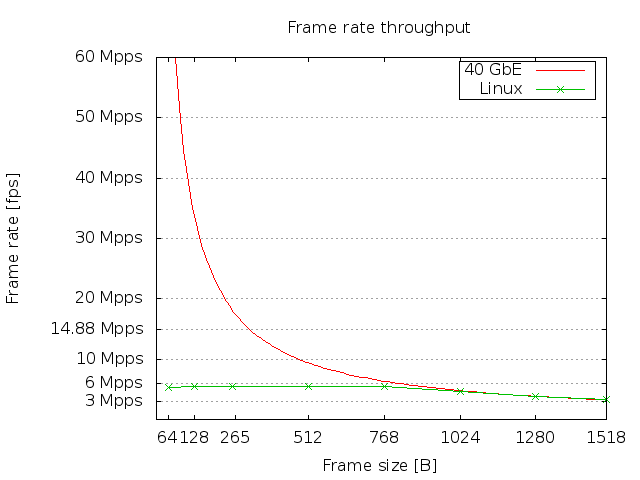
\includegraphics[width=12cm,keepaspectratio]{fig/frames.png}
\end{figure}
\noindent
The system is able to perform forwarding at nearly line rate speed with frames 1024~B and larger.
The following listing shows the actual interrupt mappings obtained from the /proc/interrupts file.
\newpage
%177:       0          0          0          0          0          0          0          0       1655  mlx4-async
\begin{landscape}
\vspace*{\fill}
\begin{lstlisting}
       CPU10      CPU11      CPU12      CPU13      CPU14      CPU15      CPU16      CPU17      CPU18
178:  298717          0          0          0          0          0          0          0          0  enp129s0-0
179:       0     294264          0          0          0          0          0          0          0  enp129s0-1
180:       0          0     291502          0          0          0          0          0          0  enp129s0-2
181:       0          0          0     296514          0          0          0          0          0  enp129s0-3
182:       0          0          0          0     302588          0          0          0          0  enp129s0-4
183:       0          0          0          0          0     294017          0          0          0  enp129s0-5
184:       0          0          0          0          0          0     294314          0          0  enp129s0-6
185:       0          0          0          0          0          0          0     302088          0  enp129s0-7
186:  402863          0          0          0          0          0          0          0          0  enp129s0d1-0
187:       0     411668          0          0          0          0          0          0          0  enp129s0d1-1
188:       0          0     416164          0          0          0          0          0          0  enp129s0d1-2
189:       0          0          0     422023          0          0          0          0          0  enp129s0d1-3
190:       0          0          0          0     421805          0          0          0          0  enp129s0d1-4
191:       0          0          0          0          0     415759          0          0          0  enp129s0d1-5
192:       0          0          0          0          0          0     402918          0          0  enp129s0d1-6
193:       0          0          0          0          0          0          0     413299          0  enp129s0d1-7
\end{lstlisting}
\vspace*{\fill}
\end{landscape}

\noindent
The RX and TX interrupts are spread across 8 CPUs.
The advantage of this mapping against the mapping done by the {\it{irqbalance}} daemon
is that it requires half the CPUs and the IRQ serving should cause fewer cache misses as well.
The listing bellow shows the cache statistics.
\begin{lstlisting}[language=TeX]
 L3MISS: L3 cache misses 
 L2MISS: L2 cache misses (including other core's L2 cache *hits*) 
 L3HIT : L3 cache hit ratio (0.00-1.00)
 L2HIT : L2 cache hit ratio (0.00-1.00)
 L3CLK : ratio of CPU cycles lost due to L3 cache misses (0.00-1.00)
 L2CLK : ratio of CPU cycles lost due to missing L2 cache (0.00-1.00)
 L3OCC : L3 occupancy (in KBytes)
 
 Core (SKT) | L3MISS | L2MISS | L3HIT | L2HIT | L3CLK | L2CLK |  L3OCC
   0    0     5799       33 K    0.82    0.24    0.19    0.18        0
   1    0      122     2488      0.95    0.15    0.03    0.14        0
   2    0      374     3928      0.90    0.19    0.00    0.00        0
   3    0        8      532      0.98    0.15    0.01    0.08       80
   4    0        6      519      0.99    0.16    0.00    0.08        0
   5    0       13      540      0.98    0.13    0.01    0.07        0
   6    0       12      552      0.98    0.14    0.01    0.07        0
   7    0       12      560      0.98    0.14    0.01    0.08      120
   8    0        9      547      0.98    0.13    0.01    0.08        0
   9    0       25      593      0.96    0.13    0.02    0.08        0
  10    1     9527     6014 K    1.00    0.51    0.00    0.14     1080
  11    1     9633     6096 K    1.00    0.52    0.00    0.14     1280
  12    1     9440     6257 K    1.00    0.53    0.00    0.15     1280
  13    1     9349     6069 K    1.00    0.54    0.00    0.14      960
  14    1     9147     6007 K    1.00    0.50    0.00    0.14     1000
  15    1     9270     6043 K    1.00    0.52    0.00    0.15     1160
  16    1     9382     6230 K    1.00    0.52    0.00    0.15     1560
  17    1     9249     6055 K    1.00    0.56    0.00    0.14      920
  18    1     1395     8002      0.83    0.15    0.29    0.29       40
  19    1      198     1129      0.82    0.12    0.13    0.14        0
  20    0      171     1042      0.84    0.08    0.07    0.11       40
  21    0       35     1176      0.97    0.16    0.02    0.17        0
  22    0       24      715      0.97    0.13    0.01    0.11       40
  23    0       18      537      0.97    0.15    0.01    0.09        0
  24    0        5      536      0.99    0.16    0.00    0.09        0
  25    0       11      533      0.98    0.14    0.01    0.08        0
  26    0       15      541      0.97    0.14    0.01    0.08        0
  27    0       11      538      0.98    0.16    0.01    0.09        0
  28    0       14      547      0.97    0.15    0.01    0.09        0
  29    0       46      672      0.93    0.12    0.03    0.10        0
  30    1      557     1200      0.54    0.34    0.03    0.01        0
  31    1      181      612      0.70    0.21    0.26    0.14       40
  32    1      192      604      0.68    0.23    0.25    0.12        0
  33    1      246      634      0.61    0.22    0.31    0.12        0
  34    1      202      622      0.68    0.22    0.28    0.15        0
  35    1      144      599      0.76    0.25    0.20    0.15        0
  36    1      127      620      0.80    0.22    0.17    0.15        0
  37    1      142      619      0.77    0.20    0.21    0.16       40
  38    1      132      685      0.81    0.11    0.13    0.15        0
  39    1      308      921      0.22    0.43    0.38    0.02      360
------------------------------------------------------------------------
 SKT    0     6730       50 K    0.87    0.21    0.03    0.04      280
 SKT    1       85 K     48 M    1.00    0.52    0.00    0.14     9720
------------------------------------------------------------------------
 TOTAL  *       92 K     48 M    1.00    0.52    0.00    0.14     N/A
\end{lstlisting}
As expected, the total cache miss count is lower with the manual IRQ mappings.
\\
The manual mappings are the best IRQ affinity settings in terms of number of CPUs used,
cache use and predictability.
